%Book project to summarize study on German language
\documentclass[12pt,a4paper,twoside]{book}
\usepackage[textwidth=16.5cm,textheight=25cm]{geometry}
\usepackage[ngerman,english]{babel}
\usepackage{amsmath,amssymb,amsfonts} % Typical maths resource packages
\usepackage{graphics}                 % Packages to allow inclusion of graphics
\usepackage{color}                    % For creating coloured text and background
\usepackage[T1] {fontenc}
\usepackage{epsfig}
\usepackage{pstricks}
\usepackage{booktabs}                 % For formal tables
\usepackage{float}
\usepackage{times}
\usepackage{fancyhdr}                 % Package used to redefine headers
\usepackage{lipsum}
\usepackage{url}
\usepackage{tipa}                     % Package to simplify the typing of pronunciation guide using IPA

\title{Vorlesungsskript zum Deutschkurs}
\author{Fernando Martins Cardoso}

\begin{document}

\thispagestyle{empty}
\newcommand{\HRule}{\rule{\linewidth}{1mm}}
\setlength{\parindent}{0mm}
\setlength{\parskip}{0mm}
 \vspace*{\stretch{1}}
 \HRule
 \begin{flushright}
  \Huge Vorlesungsskript zum Deutschkurs\\[5mm]
        \huge Fernando Martins Cardoso
 \end{flushright}
 \HRule
 \vspace*{\stretch{2}}
 \begin{center}
  \Large\textsc{München\\ 2025}
 \end{center}
 
\newpage
\topmargin 7.2in
\thispagestyle{empty}
\begin{flushright}
\textit{Fantasie ist wichtiger als Wissen, denn Wissen ist begrenzt.\\Albert Einstein}
\end{flushright}

\newpage
%Page setup as per The Latex Companion p. 85 (Geometrical dimensions of the Layout)
\hoffset -1in           % Removing standard horizontal offset
\voffset -1in           % Removing standard vertical offset
\marginparwidth 0pt     % Margin notes width
\marginparsep 0pt       % Margin notes separation
\parindent 12pt         % Paragraph indentation
\parskip 4pt            % Paragraph skip length
\topmargin 1cm          % Top margin length
\headheight 15pt        % Head height length
\headsep 20pt           % Head separation
\oddsidemargin 2.5cm    % Extra space added at the left of odd-numbered pages
\evensidemargin 2cm     % Extra space added at the left of even-numbered pages
\footskip 40pt

\chapter*{Preface}
\pagenumbering{roman}
This is a free 

\tableofcontents

\newpage
\pagenumbering{arabic}

% fancy package setup for the rest of the book:
\pagestyle{fancy}                   % Switch to the fancy page style
\fancyhf{}                          % Clear all header and footer fields
\fancyfoot[LE]{\thepage}             % Position of page numbering
\fancyfoot[RO]{\thepage}

%Chapter 1

\fancyhead[RO]{\slshape Aussprachekurs}  % Mark on right odd pages
\fancyhead[LE]{\slshape Deutschkurs}     % Mark on left even pages
\chapter*{Aussprachekurs}
\addcontentsline{toc}{chapter}{Aussprachekurs}

\begin{flushright}
\mbox{%
\begin{minipage}{0.5\textwidth}
{\textit{\footnotesize{Der Alte verliert eines der größten Menschenrechte: \\er wird nicht mehr von seines Gleichen beurteilt.}}}
\begin{flushright}
{\scriptsize{Johann Wolfgang von Goethe}}
\end{flushright}
\end{minipage}%
}
\end{flushright}

This chapter is dedicated to study the German language pronunciation. The content is based on the first chapter of the book \cite{berlitz2000}, on the Aussprachekurs from Professor Raville in \cite{raville2025}, and on the pronunciation indicated in \cite{langen2015} and \cite{wiktionary} using International Phonetic Alphabet (IPA).

\section*{Accent and pronunciation}

According to \cite{raville2025}, accent is a particular way of pronouncing certain phonemes, which can change the melody and rhythm of a particular word or phrase. While pronunciation has a more rigid structure which, even with the variation in accents, must be preserved so as not to compromise the communication process. Therefore, this material focus on German standard pronunciation (\textit{Standardaussprache}) to keep the speech clear during verbal communication.

To check the stressed\footnote{In linguistics, and particularly phonology, stress or accent is the relative emphasis or prominence given to a certain syllable in a word or to a certain word in a phrase or sentence \cite{wiki_stress}. But this accent must not be confused with the sociolinguistic meaning of accent mentioned on the previous paragraph, which is a way of pronouncing a language that is distinctive to a country, area, social class, or individual \cite{wiki_accent}.} syllable of German words, the website of the famous German dictionary Duden can be consulted at the following link \url{https://www.duden.de/}. To check phonetic transcription and etimology, Wiktionary, the free dictionary available in \url{https://en.wiktionary.org/wiki/} has an excellent database. Finally, to check pronunciation with audio recordings of native speakers, the website \url{https://www.forvo.com/} is a great option.

\section*{How to improve the pronunciation in German}

In \cite{raville2025}, the following tasks are suggested to improve pronunciation:
\begin{itemize}
    \item Always read aloud, and use a voice recorder frequently.
    \item Check your pronunciation on Google Translate or similar online translators. Do they ``understand'' you?
    \item Identify what is most challenging for you to pronounce and practice a lot until you master it.
    \item When speaking German, articulate a lot and exaggerate. This is normal in the beginning.
    \item Sing in German.
\end{itemize}

% The German Alphabet

\section*{A}

Letter name \textipa{[a]}. In words, this letter sounds like the a in \textbf{a}lgae.

Examples:
\begin{enumerate}
    \item \textbf{aus}: \textipa{[aUs]}
    \item \textbf{auf}: \textipa{[aUf]}
    \item \textbf{an}: \textipa{[an]}
    \item \textbf{aktuell}: \textipa{[aktu"El]}
\end{enumerate}

\section*{Ä}

Letter name \textipa{[a]} Umlaut, pronounced \textipa{[E:]}. In words, this letter can sound long (i.e., stressed), or short (i.e., unstressed) \cite{umlaute2021}.

Examples of long ä:
\begin{enumerate}    
    \item \textbf{Hähnchen}: \textipa{["hE:n\c{c}@n]}
    \item \textbf{Käse}: \textipa{["kE:z@]}
    \item \textbf{schläfst}: \textipa{["SlE:fst]}
    \item \textbf{Verspätung}: \textipa{[fEr"SpE:tUN]}
\end{enumerate}

Examples of short ä:
\begin{enumerate}
    \item \textbf{ändern}: \textipa{["End@rn]}
    \item \textbf{Gäste}: \textipa{["gEst@]}
    \item \textbf{Männer}: \textipa{["mEn@r]}
    \item \textbf{März}: \textipa{[mErts]}
    \item \textbf{wäscht}: \textipa{[vESt]}
\end{enumerate}

Depending on the area of Germany, ä can sound as short in words where it is usually long, e.g., \textbf{schläfst} being pronounced as \textipa{["SlEfst]}, and \textbf{später} being pronounced \textipa{["SpEt@r]}.

\section*{B}

Letter name \textipa{[be:]}. In words, this letter sounds like b before vowels, as in \textbf{b}ow. And it sounds like silent p at the end of words and before consonants, as in ma\textbf{p}.

Examples:
\begin{enumerate}
    \item \textbf{Ab}: \textipa{[ap]}
    \item \textbf{bald}: \textipa{[balt]}
    \item \textbf{bekommen}: \textipa{[be"kOm@n]}
    \item \textbf{Bier}: \textipa{[bi:r]}
    \item \textbf{Bus}: \textipa{[bUs]}
    \item \textbf{gelb}: \textipa{[gElp]}
    \item \textbf{gibt}: \textipa{[gIpt]}
    \item \textbf{habt}: \textipa{[hapt]}
    \item \textbf{halb}: \textipa{[halp]}
    \item \textbf{Obst}: \textipa{[o:pst]}
    \item \textbf{siebzehn}: \textipa{["zi:ptse:n]}
\end{enumerate}

\section*{C}

Letter name \textipa{[tse:]}. In words, this letter sounds like ts before e and i, and sounds like k before a, o and u. It is not a common letter in German language, mostly used in foreign words incorporated into German.

Examples:
\begin{enumerate}
    \item \textbf{Café}: \textipa{[ka"fe:]}
    \item \textbf{campen}: \textipa{["kEmp@n]}
    \item \textbf{Celsius}: \textipa{["tselziUs]}
    \item \textbf{Chaos}: \textipa{["ka:os]}
    \item \textbf{Curry}: \textipa{["k{\oe}ri]}
\end{enumerate}

\section*{D}

Letter name \textipa{[de:]}. In words, this letter sounds like d before vowels, as in \textbf{d}og. And it sounds like silent t at the end of words and before consonants, as in ca\textbf{t}.

Examples:
\begin{enumerate}
    \item \textbf{Bild}: \textipa{[bIlt]}
    \item \textbf{Dame}: \textipa{["da:m@]}
    \item \textbf{dämpfen}: \textipa{["dEmpf@n]}
    \item \textbf{davor}: \textipa{["da:fOr,da"fo:r]}
    \item \textbf{Freund}: \textipa{[frOYnt]}
    \item \textbf{Hand}: \textipa{[hant]}
    \item \textbf{Kind}: \textipa{[kint]}
    \item \textbf{Land}: \textipa{[lant]}
    \item \textbf{Stadt}: \textipa{[Stat]}
    \item \textbf{Versand}: \textipa{[fEr"zant]}
\end{enumerate}

\section*{E}

Letter name \textipa{[e:]}. In words, this letter sounds like Spanish or Portuguese \textbf{e}, as in abu\textbf{e}lo. But it sounds more subtle at the end of words, as in mom\textbf{e}nt.

Examples:
\begin{enumerate}
    \item \textbf{eine}: \textipa{["aIn@]}
    \item \textbf{esse}: \textipa{["Es@]}
    \item \textbf{Frage}: \textipa{["fra:g@]}
    \item \textbf{heute}: \textipa{["hOYt@]}
    \item \textbf{lese}: \textipa{["le:s@]}
    \item \textbf{Sprache}: \textipa{["Spra:x@]}
    \item \textbf{Wange}: \textipa{["vang@]}
\end{enumerate}

\section*{F}

Letter name \textipa{[Ef]}. In words, this letter sounds like f as in \textbf{f}ate or \textbf{f}riend.

Examples:
\begin{enumerate}
    \item \textbf{Fach}: \textipa{[fax]}
    \item \textbf{fegen}: \textipa{["fe:g@n]}
    \item \textbf{Feier}: \textipa{["faI@r]}
    \item \textbf{Flug}: \textipa{[flu:k]}
    \item \textbf{freundlich}: \textipa{["frOYntli\c{c}]}
    \item \textbf{Frucht}: \textipa{[frUxt]}
    \item \textbf{Fußball}: \textipa{["fu:sbal]}
\end{enumerate}

\section*{ß}

Letter name \textit{eszett} or \textit{scharfes S}. In words, this letter sounds like the ss in pa\textbf{ss}ing and comes after a long vowel or diphthong (blend of two vowel sounds in a single syllable).

According to \cite{wiki_germanalpha}, as the ß derives from a ligature of lower-case letters, it is itself exclusively lower-case. The proper transcription when it cannot be used, or when writing a word in all capital letters, is \textbf{ss} or \textbf{SS}. The ß is not used in Switzerland and Liechtenstein, where it was replaced by \textbf{ss}.

Examples:
\begin{enumerate}
    \item \textbf{außen}: \textipa{["aUs@n]}
    \item \textbf{dreißig}: \textipa{["draIsI\c{c}]}
    \item \textbf{Fuß}: \textipa{[fu:s]}
    \item \textbf{groß}: \textipa{[gro:s]}
    \item \textbf{Gruß}: \textipa{[gru:s]}
    \item \textbf{heißen}: \textipa{["haIs@n]}
    \item \textbf{schließen}: \textipa{["Sli:s@n]}
    \item \textbf{Spaß}: \textipa{[Spa:s]}
    \item \textbf{Straße}: \textipa{["Stra:s@]}
    \item \textbf{weiß}: \textipa{[vaIs]}
\end{enumerate}

When the vowel is short, the word is written with \textbf{ss}. Examples:

\begin{enumerate}
    \item \textbf{essen}: \textipa{["Es@n]}
    \item \textbf{Fluss}: \textipa{[flUs]}
    \item \textbf{gerissen}: \textipa{[g@"rIs@n]}
    \item \textbf{krass}: \textipa{[kras]}
    \item \textbf{muss}: \textipa{[mUs]}
\end{enumerate}

%%Chapter 2
\chapter*{Exemplos de tabela e figura}
\addcontentsline{toc}{chapter}{Exemplos de tabela e figura}
\fancyhead[RO]{\slshape Exemplos de tabela e figura}  % Mark on right odd pages
\fancyhead[LE]{\slshape Deutschkurs}     % Mark on left even pages

 Figura pós-formata\c{c}\~ao:
\begin{figure}[H]
    \centering
    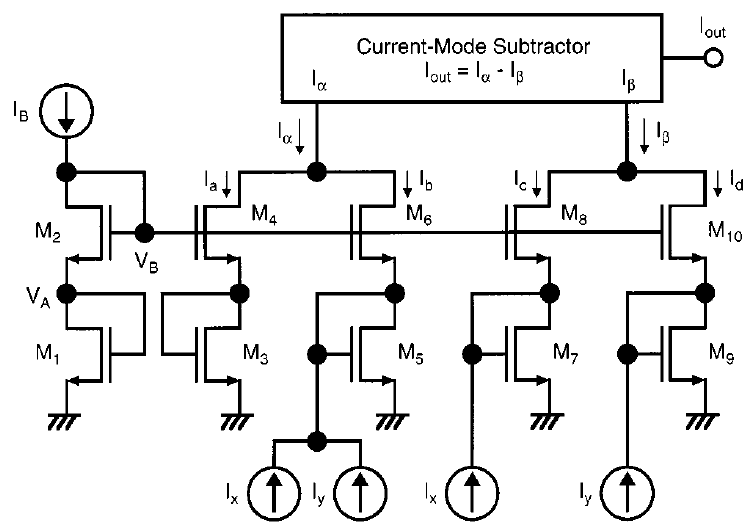
\includegraphics[width=0.5\textwidth]{figures/tanno_multiplier.png}
    \caption{\small Multiplicador de quatro quadrantes proposto em \cite{einstein1905}.\normalsize}
    \label{fig_tanno}
\end{figure}

Tabela simples:
\begin{table}[h]
    \centering
    \caption{Razões de aspecto}
    \label{tab_aspectos}
    \begin{tabular}{|l|r|r|}
    \hline
    Transistor                    & W/L ($\mu$m/$\mu$m) \\ \hline
    M$_1$ e M$_2$                 & 10/0,5              \\ \hline
    M$_3$ a M$_{10}$              & 3,5/0,5             \\ \hline
    M$_{11}$ a M$_{18}$           & 40/0,5              \\ \hline
    M$_{19}$ a M$_{22}$           & 3,5/0,5             \\ \hline
    M$_{1N}$ a M$_{4N}$           & 2,0/0,5             \\ \hline
    M$_{1P}$ a M$_{6P}$           & 20/0,5              \\ \hline
    \end{tabular}
\end{table}

\lipsum[1-25]


\bibliographystyle{plain}       % Choose a bibliography style
\bibliography{deutsch_proj_bib} % Replace with the name of your .bib file (without the .bib extension)

\end{document}
